\documentclass[aspectratio=169]{beamer}

\usepackage{graphbox}
\usepackage{array} 

\usetheme{Boadilla}
\setbeamersize{text margin left=2.3em,text margin right=2.3em}
\setbeamertemplate{bibliography item}{\insertbiblabel}
\setbeamertemplate{navigation symbols}{
  \usebeamerfont{footline}%
  \usebeamercolor[fg]{footline}%
  \footnotesize \insertframenumber/\inserttotalframenumber
  \hspace*{1.2em}
  \vspace*{.7em}
}
\setbeamertemplate{footline}{}
\definecolor{red}{HTML}{C73E1D}
\definecolor{yelloworange}{RGB}{255, 205, 0}
\definecolor{gray}{RGB}{40, 40, 40}
\definecolor{darkgray}{RGB}{30, 30, 30}
\setbeamercolor{frametitle}{bg=yelloworange, fg=black}
\setbeamercolor{normal text}{fg=gray, bg=white}
\setbeamercolor{alerted text}{fg=red}
\setbeamercolor{example text}{fg=green!50!black}
\setbeamercolor{structure}{fg=darkgray}
\parskip=10pt

\usepackage{minted}
\RecustomVerbatimEnvironment{Verbatim}{BVerbatim}{}
\newenvironment{haskell}
    {\VerbatimEnvironment\begin{minted}[escapeinside=!!]{haskell}}
    {\end{minted}}
\newenvironment{chaskell}
    {\VerbatimEnvironment\begin{center}\begin{minted}[escapeinside=!!]{haskell}}
    {\end{minted}\end{center}}
\newenvironment{slide}[1]
  {\begin{frame}[fragile,environment=slide]{\secname\ – #1}}
  {\end{frame}}
\long\def\ignore#1{}

\usepackage{amsmath}
\usepackage[utf8]{inputenc}
\usepackage{biblatex}
\addbibresource{references.bib}

\title{Generic Incremental Computation for Regular Datatypes}
\author{Jort van Gorkum}
\institute{Utrecht University}
\date{\today}

\begin{document}

\begin{frame}

\includegraphics[height=.7cm]{images/UU_logo_2021_EN_RGB.pdf}%
\vspace*{\fill}

\large \textbf{Generic Incremental Computation for Regular Datatypes}

\textcolor{yelloworange}{\rule{\textwidth}{0.2mm}}

\vspace*{0.5cm}

Jort van Gorkum

\vspace*{0.3cm}

\small \today
\end{frame}

\section{Title Explanation}

% Incremental Computation

\begin{slide}{Incremental Computation}
\centering
\large \textbf{Generic \textcolor{red}{Incremental Computation} for Regular Datatypes}

\vspace*{.5cm}
\textbf{=}
\vspace*{.5cm}

Incremental computation is an approach to improve performance by only recomputing result for changed input

\end{slide}

% Incremental Computation Example

\begin{slide}{Example Incremental Computation}
\begin{haskell}
fib :: Int -> Int
fib 0 = 0
fib 1 = 1
fib n = fib (n - 1) + fib (n - 2)
\end{haskell}
\begin{center}  
\textbf{Call Hierarchy}

\vspace*{.2cm}
\begin{minted}{text}
                  fib(4)  
               /          \
          fib(3)           fib(2)
          /   \            /   \
     fib(2)   fib(1)  fib(1)   fib(0)
     /   \
 fib(1)  fib(0)
\end{minted}
\end{center}
\end{slide}

\begin{slide}{Example Incremental Computation}

% TODO: Write how incremental computation relates to Memoization

\centering
{\huge \textit{Memoization}}

\vspace*{0.4cm}

stores the result of a computation and returns the cached result when the same input occurs again.

\end{slide}

\begin{slide}{Example Incremental Computation}
\begin{minipage}{.45\textwidth}
\begin{center}
\textbf{New Call Hierarchy}

\vspace*{.7cm}
\begin{minted}[escapeinside=!!]{text}
                  fib(4)  
               /          \
          fib(3)           !\textcolor{red}{fib(2)}!
          /   \      
      fib(2)   fib(1)
      /   \
  fib(1)  fib(0)
\end{minted}
\end{center}
\end{minipage}
\hfill
\begin{minipage}{.45\textwidth}
  \begin{center}
    \begin{table}[h]
      \begin{tabular}{ | c | c | }
        \hline
        \textbf{Function Call} & \textbf{Result} \\ 
        \hline
        fib(2) & 1 \\
        \hline
        fib(3) & 2 \\
        \hline
        fib(4) & 3 \\
        \hline
      \end{tabular}
    \end{table}
    \vspace*{0.7cm}

    \textbf{Cached Results}
  \end{center}
\end{minipage}
\end{slide}

% Generic Programming

\begin{slide}{Generic}
\centering
\large \textbf{\textcolor{red}{Generic} Incremental Computation for Regular Datatypes}

\vspace*{.5cm}
\textbf{=}
\vspace*{.5cm}

Generic refers to \textit{datatype-generic programming}, which is a form of abstraction that allows defining functions that can operate on a large class of datatypes. 

\end{slide}

% Generic Programming Example

\begin{slide}{Generic Example}
\begin{haskell}
data List a = Nil | Cons a (List a) -- Haskell Notation [] | x : [] 

length :: List a -> Int
length Nil        = 0
length (Cons _ t) = 1 + length t

data Tree a = Leaf | Node (Tree a) a (Tree a)

length :: Tree a -> Int
length Leaf _       = 1
length (Node l _ r) = 1 + length l + length r
\end{haskell}
\end{slide}

\begin{slide}{Generic Example}
\begin{chaskell}
gLength :: (Generic f) => f a -> Int
gLength = ...
\end{chaskell}

A \textit{single} \texttt{length} function can be written, that can operate on lists, trees, and many other datatypes

\vspace*{0.5cm}
\begin{haskell}
> gLength (Cons 1 (Cons 2 (Cons 3 Nil))) -- List Int
    3

> gLength (Node Leaf 1 Leaf) -- Tree Int
    3
\end{haskell}
\end{slide}

% Regular Datatypes

\begin{slide}{Regular Datatypes}
\centering
\large \textbf{Generic Incremental Computation for \textcolor{red}{Regular Datatypes}}

\vspace*{.5cm}
\textbf{=}
\vspace*{.5cm}

Regular datatypes are recursive datatypes, which can only recurse into themselves, such as lists, binary trees, etc. 

\end{slide}

% Regular Datatypes Example

\begin{slide}{Regular Datatypes Example}
\textbf{Regular Datatypes}

\begin{haskell}
data List a = Nil | Cons a (List a)

data Tree a = Leaf | Node a (Tree a) (Tree a)
\end{haskell}

\vspace*{0.5cm}
\textbf{\textcolor{red}{Not} Regular Datatypes}

\begin{haskell}
data Tree a = Empty | Node a (Forest a)

data Forest a = Nil | Cons (Tree a) (Forest a)
\end{haskell}
\end{slide}

\begin{slide}{Summary}
summary
\end{slide}

\section{Goal}

\begin{slide}{What does this solve?}

Goal: implement an incremental algorithm which performs better than the non-incremental algorithm for large regular datatypes

\end{slide}

% Example

\begin{slide}{Example Problem with Memoization}
\begin{haskell}
data Tree a = Leaf a | Node (Tree a) a (Tree a)

sumTree :: Tree Int -> Int
sumTree (Leaf x)     = x
sumTree (Node l x r) = x + sumTree l + sumTree r

exampleTree = Node (Node (Leaf 1) 3 (Leaf 2)) 5 (Node (Leaf 1) 3 (Leaf 2))
\end{haskell}

\begin{center}
\textbf{Visual representation}

\begin{minipage}{.1\textwidth}
\texttt{sumTree(}
\end{minipage}
\begin{minipage}{.2\textwidth}
\begin{center}
\begin{minted}{text}
     5 
   /   \
  3     3
 / \   / \
1  2   1  2
\end{minted}
\end{center}
\end{minipage}
\begin{minipage}{.1\textwidth}
\texttt{) = 17}
\end{minipage}
\end{center}
\end{slide}

%  -------------------

\begin{slide}{Example Problem with Memoization}
  
{\Large \textbf{Memoized} version of the \texttt{sumTree}}

\begin{minipage}{.45\textwidth}
\begin{center}
\textbf{Example Tree}

\vspace*{0.4cm}
\begin{minted}[escapeinside=!!]{text}
     5 
   /   \
  3     !\textcolor{red}{3}!
 / \   !\textcolor{red}{/ \texttt{\symbol{92}}}!
1  2   !\textcolor{red}{1  2}!
\end{minted}
\end{center}
\end{minipage}
\hfill
\begin{minipage}{.45\textwidth}
\begin{center}
\begin{tabular}{ | m{0.45\textwidth} | >{\centering\arraybackslash} m{1cm} | }
\hline
\textbf{Tree} & \textbf{Result} \\ 
\hline
\vspace{0.3cm}
\begin{minipage}[t]{.2\textwidth}
\begin{minted}{text}
      5 
    /   \
   3     3
  / \   / \
 1  2   1  2
\end{minted}
\end{minipage}
\vspace*{0.3cm} & 17 \\
\hline
\vspace{0.3cm}
\begin{minipage}[t]{.2\textwidth}
\begin{minted}{text}
      3 
     / \ 
    1   2
\end{minted}
\end{minipage}
\vspace{0.5em}  & 6 \\
\hline
\end{tabular}
\vspace*{0.7cm}

\textbf{Cached Results}
\end{center}
\end{minipage}
\end{slide}

\section{Solution}

\begin{slide}{Using Hash function}
A \textit{hash function} is a process of transforming input into an arbitrary fixed-size value (i.e., digest), where the same input always generates the same output

\begin{center}
\begin{minted}[escapeinside=!!]{text}
     5 
   /   \
  3     3       ->    1da16c7c48e429b4ad6e6c88d941d2bd
 / \   / \    
1  2   1  2                       !\textcolor{red}{Digest}!  
\end{minted}
\end{center}
\end{slide}

% \begin{slide}{Implementation Hash function}
% \begin{haskell}
% class Hashable a where
%   hash :: a -> Digest

% instance Hashable a => Hashable (Tree a) where
%   hash (Leaf x)     = concatDigest [hash "Leaf", hash x]
%   hash (Node l x r) = concatDigest [hash "Node", hash l, hash x, hash r]
% \end{haskell}
% \end{slide}

\begin{slide}{Storing the Digests}
A \textit{Merkle Tree} is a data structure which integrates the \textit{digests}, which represents the internal structure, within the data structure

\vspace*{0.4cm}
\begin{haskell}
data TreeH a = LeafH Digest a
             | NodeH Digest (TreeH a) a (TreeH a)


merkle :: Tree Int -> TreeH Int
merkle l@(Leaf x)     = LeafH (hash l) x
merkle b@(Node l x r) = NodeH (hash b) l' x r'
  where
    l' = merkle l
    r' = merkle r
\end{haskell}
\end{slide}

\begin{slide}{Using Digests} 
\begin{haskell}
sumTreeInc m (LeafH d x) = case lookup d m of
  Just z  -> (z, m)
  Nothing -> (x, insert d x m)

...
\end{haskell}

\begin{haskell}
SumTreeInc 
\end{haskell}
\end{slide}

\begin{slide}{Updating the Input}
The \textit{Zipper} is a technique for keeping track of how the data structure is being traversed through

\begin{center}
\begin{minted}[escapeinside=!!]{text}
     !\textcolor{red}{5}!                           5     
   /   \                           \    
  3     3      ->      !\textcolor{red}{3}!            3    
 / \   / \            / \          / \  
1  2   1  2          1   2        1   2 
\end{minted}

\textbf{Go to the left Subtree of the Tree}
\end{center}

Using the Zipper, we can traverse through the data structure and update the values where needed. And to restore the tree, we go up and while we are going up, we update the digests of the nodes.
\end{slide}

% \begin{slide}{Zipper - Left}


% \vspace*{0.4cm}
% \begin{haskell}
% left :: Loc a -> Loc a
% left (Node l x r, cs) = (l, (L r x):cs)
% \end{haskell}
% \end{slide}

% \begin{slide}{Zipper - Right}
% \begin{center}
% \begin{minted}[escapeinside=!!]{text}
%      !\textcolor{red}{5}!                    5     
%    /   \                 /           
%   3     3      ->       3          !\textcolor{red}{3}!  
%  / \   / \             / \        / \ 
% 1  2   1  2           1   2      1   2
% \end{minted}

% \vspace*{0.4cm}
% \begin{haskell}
% right :: Loc a -> Loc a
% right (Node l x r, cs) = (r, (R l x):cs)
% \end{haskell}
% \end{center}
% \end{slide}

% \begin{slide}{Zipper - Up}
% \begin{center}
% \begin{minted}[escapeinside=!!]{text}
%     5                        !\textcolor{red}{5}!        
%    /                       /   \           
%   3          !\textcolor{red}{3}!     ->     3     3      
%  / \        / \          / \   / \     
% 1   2      1   2        1  2   1  2   
% \end{minted}

% \vspace*{0.4cm}
% \begin{haskell}
% up :: Loc a -> Loc a
% up (t, (L r x):cs) = (Node l x r, cs)
% up (t, (R l x):cs) = (Node l x r, cs)
% \end{haskell}
% \end{center}
% \end{slide}

\section{Generic Programming}

\begin{slide}{Pattern Functors}
\begin{haskell}
data U r         = U                 -- Empty constructor
data I r         = I r               -- Recursive call
data K a r       = K a               -- Constant
data (f :+: g) r = L (f r) | R (g r) -- Sums (Choice)
data (f :*: g) r = (f r) :*: (g r)   -- Products (Combine)
\end{haskell}

\begin{haskell}
type instance PF (Tree a) = K a                -- Leaf
                         :+: (I :*: K a :*: I) -- Node
\end{haskell}
\end{slide}

\begin{slide}{Merkle}
\begin{haskell}
type Merkle f = Fix (f :*: K Digest)

class Hashable f where
  hash :: f (Merkle g) -> Digest

instance ...

merkle ...
\end{haskell}
\end{slide}

\section{Experiments}

\begin{slide}{Method}
\textbf{Three functions:}
\begin{itemize}
  \item \texttt{Cata Sum} 
  \begin{itemize}
    \item Non-incremental algorithm (which computes sumTree)
  \end{itemize}
  \item \texttt{Generic Cata Sum}
  \begin{itemize}
    \item Incremental algorithm with an empty cache
  \end{itemize}
  \item \texttt{Incremental Cata Sum}
  \begin{itemize}
    \item Incremental algorithm with a filled cache
  \end{itemize}
\end{itemize}

\textbf{Three scenarios:}
\begin{itemize}
\item{\makebox[2.5cm]{Worst case:\hfill}}   updates the lowest left leaf with a new leaf
\item{\makebox[2.5cm]{Average case:\hfill}} updates a node in the middle of the data structure with a new leaf
\item{\makebox[2.5cm]{Best case:\hfill}}    updates the left child of the root-node with a new leaf
\end{itemize} 

\end{slide}

\begin{slide}{Results - Execution Time}
  \begin{figure}[H]
    \begin{minipage}{.32\textwidth}
      \centering
      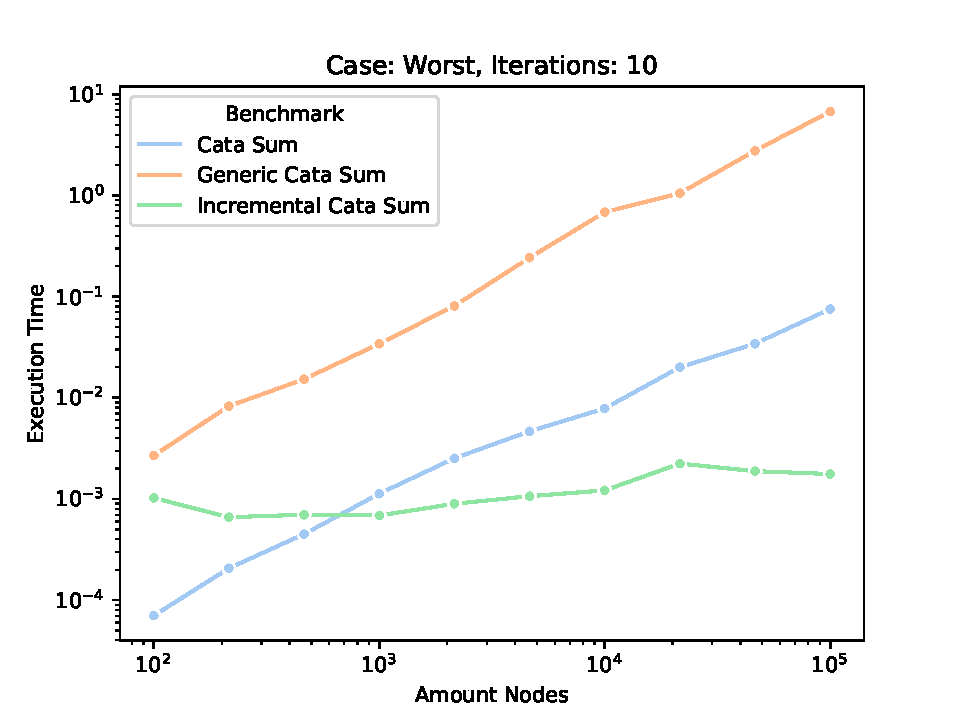
\includegraphics[width=\textwidth]{images/time/Worst/10/all_benchmarks.pdf}
    \end{minipage}
    \begin{minipage}{.32\textwidth}
      \centering
      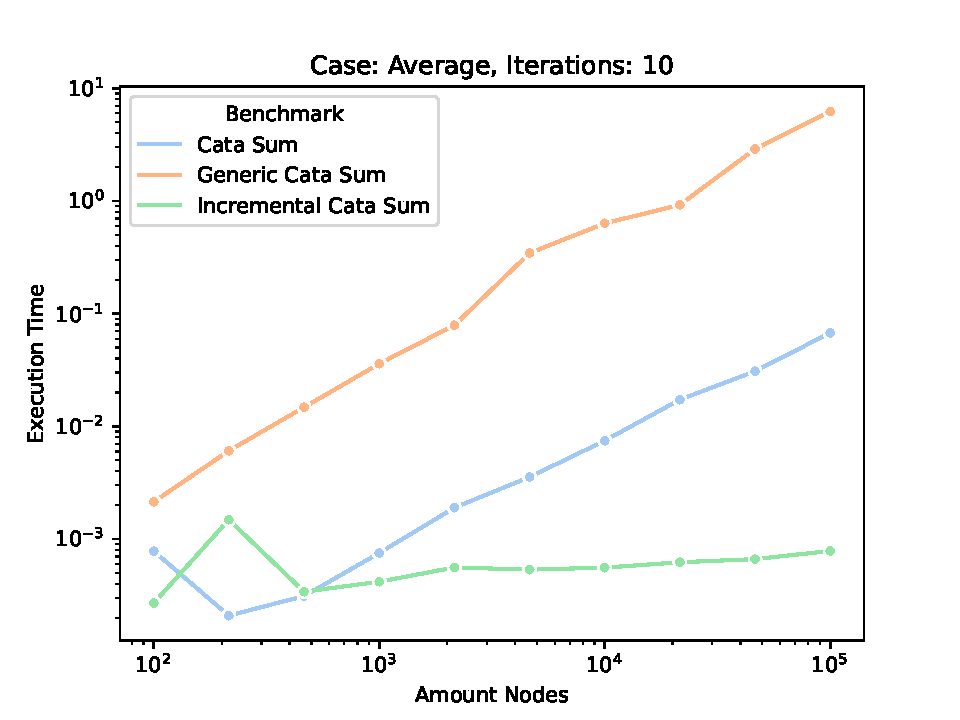
\includegraphics[width=\textwidth]{images/time/Average/10/all_benchmarks.pdf}  
    \end{minipage}
    \begin{minipage}{.32\textwidth}
      \centering
      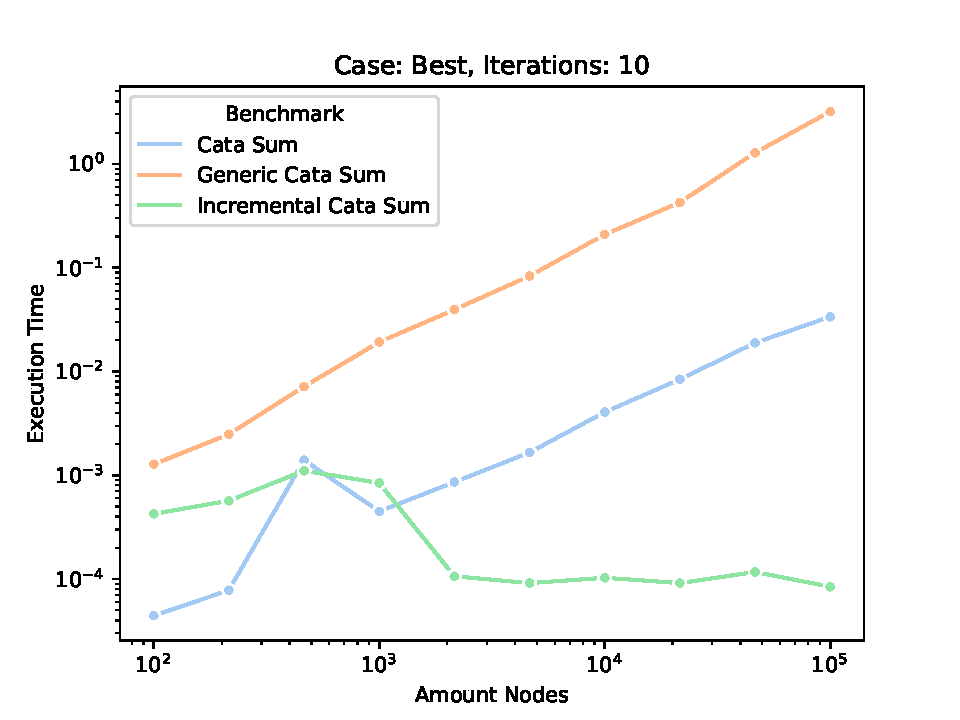
\includegraphics[width=\textwidth]{images/time/Best/10/all_benchmarks.pdf}  
    \end{minipage}
    \caption{The execution time over 10 executions for the Worst, Average and Best case.}
    \label{fig-exec-time-no-policy}
  \end{figure}
\end{slide}

\begin{slide}{Results - Memory Usage}
\begin{figure}[H]
  \begin{minipage}{.32\textwidth}
    \centering
    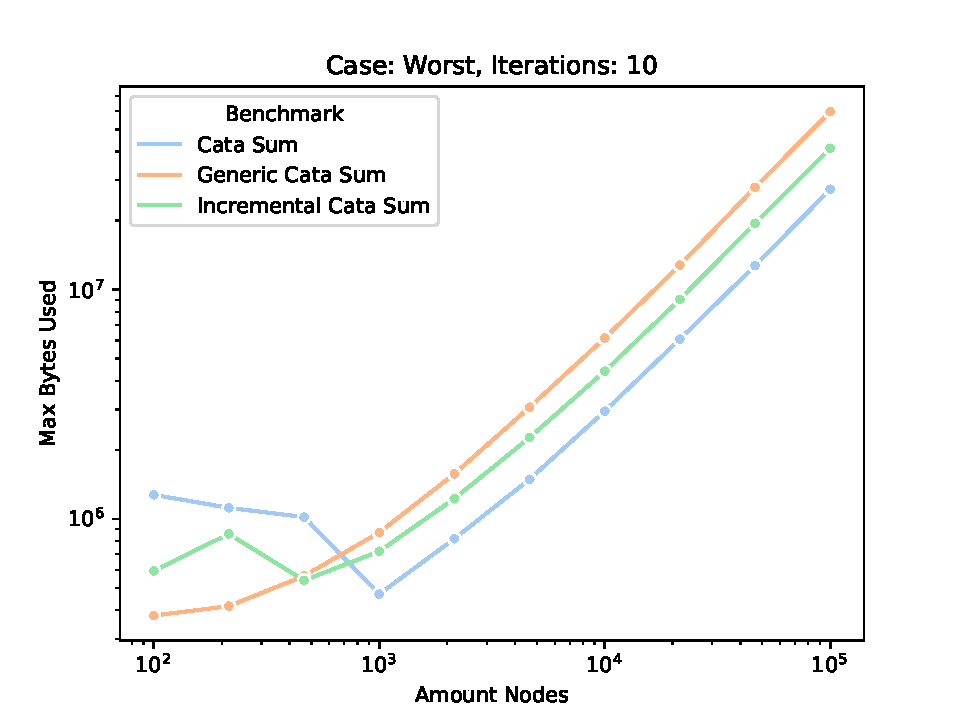
\includegraphics[width=\textwidth]{images/memory/Worst/10/all_benchmarks.pdf}  
  \end{minipage}
  \begin{minipage}{.32\textwidth}
    \centering
    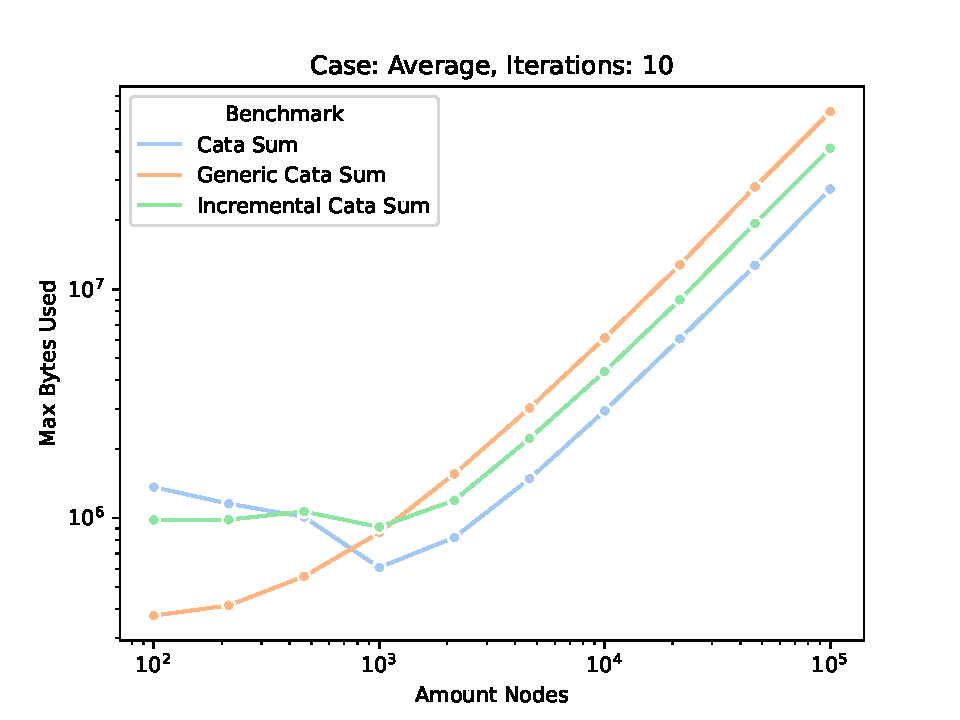
\includegraphics[width=\textwidth]{images/memory/Average/10/all_benchmarks.pdf}  
  \end{minipage}
  \begin{minipage}{.32\textwidth}
    \centering
    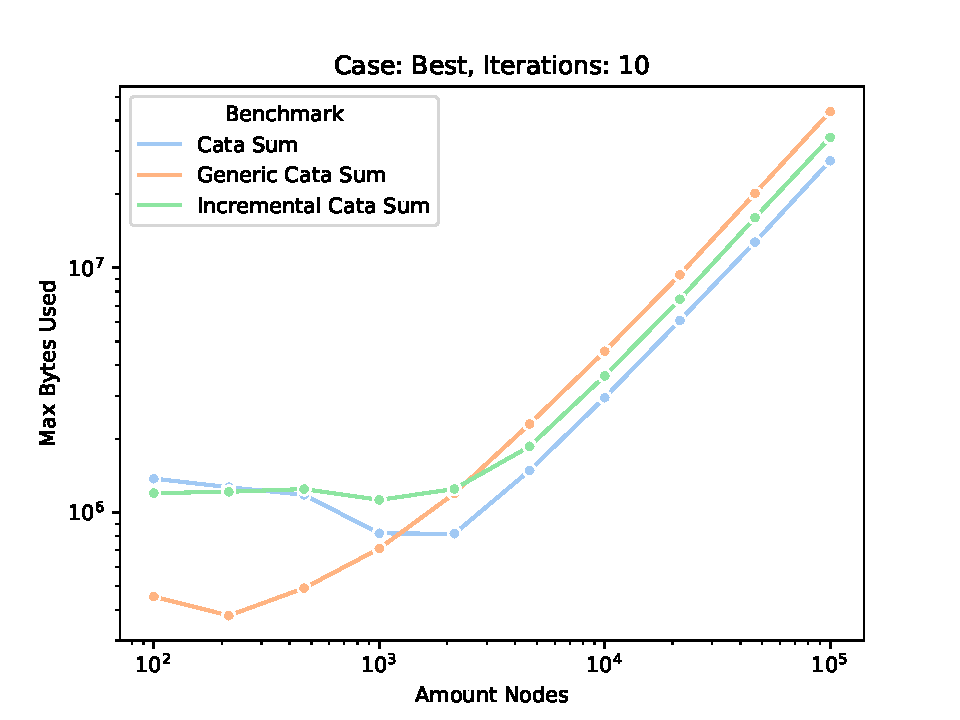
\includegraphics[width=\textwidth]{images/memory/Best/10/all_benchmarks.pdf}  
  \end{minipage}
  \caption{The max-bytes-used over 10 executions for the Worst, Average and Best case.}
  \label{fig-mem-usage-no-policy}
\end{figure}
\end{slide}


\section{Conclusion}

\begin{slide}{What I skipped for time}
\begin{itemize}
  \item The explanation of fixed-point
  \item Implementation of the generic Zipper
  \item Cache management
  \item Future work
  \item Explained what generic library is chosen and why it was chosen
\end{itemize}
\end{slide}

\begin{slide}{Summary}
\begin{itemize}
  \item We have implemented an efficient incremental algorithm over regular datatypes
  \item The incremental algorithm is faster than the non-incremental version when the data structure contains more than $10^3$ nodes
  \item We introduced the pattern synonyms to improve the developer experience to almost the same
  level as the non-incremental implementation
  \item However, the initial pass of the incremental algorithm is a lot slower than the non-incremental version. Therefore, the incremental algorithm needs to be performed a lot (with small changes), before being overall faster than the non-incremental version.
\end{itemize}
\end{slide}

% \begin{frame}{References}
% \printbibliography
% \end{frame}

\end{document}